\documentclass[10pt]{article}
\usepackage[utf8]{inputenc}
\usepackage[T1]{fontenc}
\usepackage{graphicx}
\usepackage{appendix}
\usepackage[french]{babel}
\usepackage{fancyhdr}
\usepackage{geometry}
\geometry{hmargin=3cm,vmargin=3.5cm}
\usepackage{enumitem}
\usepackage{listings}
\usepackage{subcaption}
\usepackage{amsmath}
\graphicspath{{./img/}}
\lstset{ %
  backgroundcolor=\color{white},   % choose the background color; you must add \usepackage{color} or \usepackage{xcolor}
  basicstyle=\small,               % the size of the fonts that are used for the code
  breakatwhitespace=false,         % sets if automatic breaks should only happen at whitespace
  breaklines=true,                 % sets automatic line breaking
  captionpos=b,                    % sets the caption-position to bottom
  commentstyle=\color{blue},      % comment style
%  escapeinside={\%*}{*)},          % if you want to add LaTeX within your code
  extendedchars=true,              % lets you use non-ASCII characters; for 8-bits encodings only, does not work with UTF-8
  frame=single,                    % adds a frame around the code
  keepspaces=true,                 % keeps spaces in text, useful for keeping indentation of code (possibly needs columns=flexible)
%  keywordstyle=\color{blue},       % keyword style
  language=C,                    % the language of the code
  numbers=left,                    % where to put the line-numbers; possible values are (none, left, right)
  numbersep=5pt,                   % how far the line-numbers are from the code
  numberstyle=\tiny\color{black},  % the style that is used for the line-numbers
  rulecolor=\color{black},         % if not set, the frame-color may be changed on line-breaks within not-black text (e.g. comments (green here))
  showspaces=false,                % show spaces everywhere adding particular underscores; it overrides 'showstringspaces'
  showstringspaces=false,          % underline spaces within strings only
  showtabs=false,                  % show tabs within strings adding particular underscores
  stepnumber=1,                    % the step between two line-numbers. If it's 1, each line will be numbered
  tabsize=2,                       % sets default tabsize to 2 spaces
}
\usepackage{hyperref}
\hypersetup{colorlinks=true}

\pagestyle{fancy}

\renewcommand{\sectionmark}[1]{ \markright{#1}{} }

\lhead{}
\rhead{}
\lfoot{ENSEIRB-MATMECA}
\rfoot{PRCD}
\renewcommand{\headrulewidth}{0.pt}
\renewcommand{\footrulewidth}{0.4pt}


\title{TDP1}
\author{Arnaud Durocher, Alexandre Honorat}
\date{\today}

\begin{document}
%\tableofcontents
%\newpage

\thispagestyle{empty}


%\begin{center}
%
\includegraphics{enseirb_inp.png}
%\end{center}
%
%\vspace{\stretch{1}}
\hrule
\begin{flushleft}
\Huge{\textbf{TDP4 - Utilisation de MPI}}\\
\textit{Lancer de Rayons}
\end{flushleft}
\begin{flushright}
\huge\textbf{Rapport}\\
\end{flushright}
\hrule

\vspace{80pt}
\noindent\textbf{Élèves :}
\emph{Alexandre Honorat}, \emph{Elouan Keryell-Even}\\
\\
\noindent\textbf{Responsable :}
\emph{Astrid Casadei}\\


\vspace{60pt}
\normalsize
\begin{center}
  Troisième année, filière informatique, option PRCD\\
  Date : \today\\
  Enseirb-Matmeca
\end{center}
\vspace{50pt}

%% -*- eval: (flyspell-mode 1); -*-

\chapter{Introduction}
%\addcontentsline{toc}{chapter}{Introduction}

Un des aspects de la recherche informatique consiste à améliorer des programmes afin de rendre leur temps d'exécution plus rapide, il s'agit du \emph{calcul haute performance} (ou HPC, pour High Performance Computing). 
%Les performances -- en matière de temps d'exécution -- sont primordiales par exemple pour les codes de simulation numérique dédiés à la météorologie qui calculent les prévisions du lendemain, où bien entendu la simulation doit donc s'être terminée en moins d'une nuit. 
Dans ce cadre le stage a porté sur la génération automatique de certains de ces programmes améliorés. 
Les sections suivantes présentent brièvement quelques rappels sur les problématiques HPC, ainsi que l'objectif du stage : l'adaptation automatique d'une certaine catégorie de problèmes au matériel prévu pour le HPC. Le chapitre $2$ précise plus particulièrement ces problématiques et l'objectif tandis que le chapitre $3$ se concentre sur le travail réalisé. Le chapitre $4$ en propose une évaluation et est suivi par la conclusion. 


\section{Parallélisation de programmes}

Diverses techniques existent pour améliorer les performances d'un programme et plus particulièrement de son temps d'exécution. Deux aspects peuvent entrer en compte : les algorithmes utilisés dans le programme ainsi que le matériel qui l'exécute. Le facteur limitant à améliorer en priorité est alors le matériel, car il influe sur la nature des algorithmes pouvant être utilisés.

La solution la plus simple pour améliorer les performances consisterait à se baser uniquement sur la loi de Moore, c'est-à-dire sur le fait que les capacités du matériel sur lequel le programme est exécuté sont doublées tous les ans. Or cette loi exponentielle n'est maintenant plus valable puisque la fréquence d'horloge des processeurs modernes stagne depuis quelques années à une valeur proche de $3$ GHz. 
%C'est cette fréquence d'horloge qui impose au matériel (si celui-ci est constitué de cet unique processeur) le nombre d'opérations qu'il va pouvoir effectuer en une seconde. Puisque la fréquence n'augmente plus, le nombre d'opérations par seconde pour ce type de matériel ne peut plus augmenter non plus, aucun gain de rapidité d'exécution n'est alors possible.

%La première solution s'appuyait ainsi sur l'augmentation de la fréquence, c'est-à-dire de la rapidité de chaque opération sachant qu'une seule est faite à la fois. Au lieu d'augmenter la rapidité des opérations, 
Une solution est d'augmenter le nombre d'opérations effectuées \emph{en même temps} par un processeur, ce qui est l'introduction du parallélisme dans le matériel.
%Celui-ci peut s'effectuer de plusieurs manières : à l'intérieur et à l'extérieur du processeur. À l'intérieur,
Il s'agit soit de subdiviser les instructions en  micro-instructions afin de créer un pipeline (ainsi une instruction peut commencer immédiatement après la fin de la première micro-instruction de l'instruction précédente), soit de dupliquer certains composants de l'architecture afin d'exécuter plusieurs instructions sur à la fois, soit enfin l'application de la même instruction sur plusieurs données à la fois. Les processeurs modernes intègrent tous ces trois technologies : le pipeline d'instructions, l'architecture nommée \emph{superscalaire}, et les calculs dits \emph{vectoriels}.
%À l'extérieur il s'agit de connecter plusieurs processeurs les uns avec les autres, tous participant aux calculs nécessités par le programme de base. Différentes manières de relier les processeurs existent, ils peuvent alors être appelés des cœurs ; dans toute la suite du rapport, un processeur est synonyme d'un ensemble de cœurs connectés entre eux par de la mémoire cache hiérarchique en accès uniforme\footnote{Cette notion sera explicitée au point \ref{sec:stencil_base}.}.
Les processeurs peuvent eux-mêmes être répliqués dans leur ensemble, soit sur une même surface de silicium (processeurs multicœurs), soit distinctement et alors reliés par un bus (multiprocesseurs), soit encore par une combinaison de ces deux techniques.
Enfin en dehors des processeurs classiques -- ou \emph{centraux}, abrégés en CPU -- existent aussi des processeurs graphiques -- dénommés GPU --, qui contiennent beaucoup de cœurs mais exécutent obligatoirement tous la même instruction en même temps. Bien sûr les deux types peuvent coexister sur une même machine.

La nature du matériel (et non seulement ses capacités d'ordre physique comme la fréquence d'horloge) nécessite une conception des algorithmes en adéquation (par exemple pour utiliser le côté superscalaire). 
%cela induit des modifications dans la façon de transcrire les algorithmes (par exemple pour utiliser le côté superscalaire), ainsi que dans les algorithmes eux-mêmes qui ne sont parfois plus du tout adaptés (notamment à cause des communications entre les processeurs, inexistantes auparavant). 
Écrire un programme destiné à une machine parallèle impose donc d'avoir des algorithmes souvent très spécifiques à la configuration de la machine d'exécution, ce qui est d'autant plus complexe avec les architectures des machines actuelles de plus en plus hétérogènes, et peut poser des problèmes de portabilité des applications.

\section{\'Ecriture de code parallèle}

%Les algorithmes étant souvent spécifiques au type de parallélisme et à l'architecture de la machine cible, les langages permettant d'écrire des programmes parallèles automatisent difficilement la génération de codes parfaitement adaptés à la machine cible. En pratique la plupart des langages modernes permettent l'expression du parallélisme sans le découvrir eux-même ; certains outils aident à écrire du code parallèle mais ils sont souvent expérimentaux et nécessitent alors que le code automatiquement produit soit vérifié avant d'être compilé\footnote{Lors de la transcription d'un problème en informatique, il est d'abord nécessaire de transcrire le problème vers un langage informatique (le code) -- compréhensible par les humains -- qui est alors \emph{compilé} par un programme préexistant (le compilateur) qui le transforme en fichier binaire exécutable -- compréhensible par \emph{la} machine.}.

Le procédé classique consiste à premièrement décrire le problème de manière algorithmique, deuxièmement à le transcrire dans un langage de programmation donnée -- et utiliser les outils natifs du langage ou alors les bibliothèques spécifiques pour le parallélisme -- et troisièmement à compiler le code écrit à l'étape précédente grâce à différents outils internes au compilateur. Les deux premières étapes sont réalisées par le développeur, à qui il convient de faciliter la tâche. 

Les difficultés inhérentes à la production d'un programme parallèle sont de plusieurs natures, notamment l'identification des sections parallèles et de celles obligatoirement séquentielles, ainsi que la gestion des communication et l'utilisation de toutes les ressources disponibles sur la matériel. L'identification des régions parallélisables ou non dépend de l'algorithme utilisé pour résoudre le problème voulu. Un programme bien parallélisé réduit au maximum le nombre d'opérations qui sont exécutées séquentiellement, afin que la majeure partie du temps d'exécution soit passée dans des sections parallèles où toute la puissance de la machine parallèle est utilisée. Par ailleurs il est essentiel de gérer les communications entre les différents processeurs afin que des calculs puissent être effectués pendant les communications ; on parle alors du recouvrement des communications. Enfin il convient d'utiliser le plus de ressources possibles sans que cette utilisation n'entraîne d'effort trop important, par exemple si de nombreuses parties de l'algorithme nécessitent une synchronisation de tous les processeurs -- ce qui est très coûteux en temps.

Actuellement c'est au programmeur qu'incombent presque toutes les tâches de parallélisation\footnote{En ce qui concerne les capacités des compilateurs, \textsf{gcc} comprend les directives de la bibliothèque \textsf{OpenMP}, mais ne les trouve pas automatiquement (bien qu'elles soient souvent très simples) et c'est donc au programmeur de les écrire. En revanche les compilateurs modernes sont capables d'exploiter eux-mêmes la caractère superscalaire d'un processeur, mais pas toujours de manière optimale. De même certains calculs vectoriels peuvent être détectés automatiquement, mais ils sont le plus souvent déclenchés via des fonctions spécifiques appelées par le développeur.}. %, or cela nécessite beaucoup de compétences, de temps, et de tests avant de parvenir à un résultat acceptable. S'il n'est pas toujours possible de découvrir le parallélisme automatiquement, il n'est pas non plus toujours facile de savoir où le décrire. Alors que 
Certaines options sont très proches du processeur (comme les capacités vectorielles) et doivent être gérées de manière assez fines, d'autres peuvent être prises en charge à un plus haut-niveau comme le lancement de plusieurs procédures distinctes en parallèle (a priori chacune des procédures étant alors associée à un processeur libre). %Cela amène à une hiérarchisation du parallélisme, ce qui complique encore plus la tâche du programmeur.
Par ailleurs certains paramètres du programme peuvent êtres calculés lors de la compilation -- paramètres statiques -- et d'autres uniquement lors de l'exécution -- paramètres dynamiques. Or pour améliorer la rapidité du programme, il est souhaitable de limiter les calculs lors de l'exécution. Lorsque le programmeur écrit un code en HPC, il espère donc avoir le plus possible de paramètres statiques, selon les possibilités du compilateur et du langage. 

Une des problématiques du parallélisme est donc de faciliter l'écriture de programme, soit en découvrant automatiquement le parallélisme -- ce qui est plutôt difficile -- , soit en fournissant au programmeur des outils adaptés -- ce qui est un peu plus facile.

\section{Choix du niveau d'expression du parallélisme}

%Pour écrire un programme informatique résolvant un problème donné, il est nécessaire de passer par de nombreuses étapes intermédiaires qui sont tout autant de stades où le parallélisme peut être décrit. De très nombreuses possibilités existent et nous ne les présenteront pas en intégralité ici. 

Compte-tenu de la complexité de l'écriture de code parallèle, des outils spécifiques ont été mis en place afin de faciliter le développement de tels programmes. Or ces outils -- langages, bibliothèques, ou compilateur -- sont rares et souvent trop spécifiques ou au contraire trop généraux. L'objectif du stage est donc de développer un nouvel outil adapté à un certain type de problèmes pour lequel peu d'outils existent et ne sont pas adaptés à la configuration hétérogène des machines actuelles.

Introduire un nouveau langage dédié au parallélisme est complexe car il faut non seulement développer le compilateur et les bibliothèques standards associés , mais aussi le rendre simple à utiliser et si possible pas trop éloigné des autres paradigmes dominants afin de faciliter son appréhension. D'un autre côté garder les langages existants implique de modifier les compilateurs pour qu'ils découvrent automatiquement les possibilités de parallélisation, ce qui est difficile à mettre en œuvre -- à cause de la complexité même de trouver le parallélisme, et à cause de la complexité des compilateurs modernes.
%Les deux solutions existent actuellement avec un succès mitigé\footnote{Ce constat est difficile à vérifier, mais à titre d'exemple les langages intrinsèquement parallèles que sont \textsf{Chapel} ou \textsf{Cilk} voire \textsf{Erlang} ne sont pas enseignés dans la filière PRCD de l'Enseirb-Matmeca, probablement car ils ne sont pas suffisamment répandus. Par ailleurs pour les capacités des compilateurs, \textsf{gcc} comprend les directives de la bibliothèque \textsf{OpenMP}, mais ne les trouve pas automatiquement (bien qu'elles soient souvent très simples), en revanche les compilateurs modernes sont souvent capables d'exploiter eux-mêmes la caractère superscalaire d'un processeur.}.

%Dans le cadre du stage, nous nous sommes alors plutôt intéressés aux possibilités d'un Domain Specific Embedded Language (DSEL, équivalent de \emph{langage spécifique embarqué} en français) qui permet une charge de développement moindre, ainsi qu'une appréhension rapide. En effet il s'agit alors d'une bibliothèque fournie au programmeur dans un langage courant préexistant, ne comportant que quelques fonctions reprenant uniquement les paradigmes dont le programmeur a besoin pour résoudre un type de problème spécifique, et se basant sur des bibliothèques performantes préexistantes. 
Nous avons donc décidé de développer une approche basée sur un Domain Specific Embedded Language (DSEL, équivalent de \emph{langage spécifique embarqué} en français) sous la forme d'une bibliothèque, avec comme objectifs de faciliter la prise en main du programmeur et de réduire sa charge de développement, tout en préservant ou en améliorant les performances de ses programmes.
% à recaser plus tard
%Le DSEL se différencie d'un DSL (équivalent de \emph{langage spécifique}) par le fait qu'il est disponible au sein d'un langage général, et permet donc potentiellement au développeur d'effectuer des tâches connexes à la résolution du problème dans un seul et même langage. Il peut ainsi utiliser plusieurs DSEL dans le même code, et donc résoudre des problèmes complexes avec un formalisme adapté à chacun d'entre eux (et par là-même avoir de meilleures performances). Le DSEL est ainsi une solution intermédiaire efficace, qui nous a semblé adaptée à l'objectif du stage qui est la parallélisation automatique d'une catégorie spécifique de programmes. 
Plutôt que de focaliser ce DSEL sur un type spécifique de parallélisme, ou sur un paradigme comme le font de nombreux outils, ce DSEL est focalisé sur une catégorie de problèmes et doit permettre de cacher justement tout ce qui relève du parallélisme.




\section{Protocole d'évaluation}

Cette partie décrit la manière dont nous avons procédé afin d'avoir une analyse correcte de nos algorithmes. D'une part nous avons procédé à des tests de validation afin de s'assurer que les algorithmes analysés étaient bien corrects, et d'autre part nous avons effectué des mesures sous la forme de \emph{benchmarks} afin d'analyser quantitativement les performances.

\subsection{Tests de vérification}

Les test de vérification s'assurent que les algorithmes analysés sont corrects, en mesurant l'écart entre les résultats obtenus et les résultats attendus. Dans cette partie nous détaillerons pourquoi et comment nous avons effectué ces tests, et enfin nous nous intéresserons aux améliorations que l'on pourrait y apporter.


\subsubsection{Intérêt dans le cadre du TDP}

Il est important de vérifier l'implémentation des algorithmes implémentés par des tests afin que le résultat soit correct. Cependant, dans le cadre de ce TDP, nous ne nous intéressons pas particulièrement à la précision des réponses données, mais plutôt aux manipulations de données effectuées par les algorithmes. 

Dans tous les cas, afin de comparer nos algorithmes avec des algorithmes d'autres librairies standard, il est nécessaire qu'ils résolvent les mêmes problèmes. Les valeurs trouvées lors des benchmarks n'auraient aucune valeur si l'algorithme ne calculaient pas le bon résultat.

De plus, ces tests nous permettent de vérifier que les optimisations successives ne changent pas les valeurs calculées en sortie. Des optimisations qui rendent l'algorithme invalide ne sont en effet pas intéressantes.

    
\subsubsection{Mise en \oe uvre}

Les tests mis en oeuvre sont des tests comparatifs avec des librairies système. Les résultats des routines que nous avons implémentées sont comparés aux résultats d'une librairie système. La librairie principalement utilisée est l'implémentation d'Intel \textsf{MKL}. Nous avons aussi essayé avec \textsf{cblas} de \textsf{Netlib} et \textsf{OpenBlas}. Les routines testées sont les diverses implémentations de \texttt{ddot} et \texttt{dgemm}. 

Les entrées utilisées sont générées aléatoirement à chaque exécution des tests, et les résultats sont comparés avec un résultat de référence par erreur relative. On calcule le résultat pour une entrée aléatoire, à la fois avec la routine de référence et avec la routine à tester. Ensuite nous comparons les résultats obtenus en calculant l'erreur relative pour chaque élément; si elle est inférieure à un certain seuil, nous considérons que les résultats sont égaux. La valeur du seuil choisie est de $10e^{-06}$, afin de vérifier que les valeurs calculées ne sont pas trop éloignées de la valeur réelle sans se préoccuper d'éventuelles erreurs d'instabilité numérique.

Cette comparaison est effectuée sur des matrices générées aléatoirement, elle permet donc de tester la validité de la librairie pour un certain nombre de conditions différentes (taille de matrice, écart d'échelle entre les éléments), et ce de manière simple et automatisée.

\subsubsection{Réflexions}
  
La vérification par comparaison avec une autre librairie est discutable. D'une part la librairie prise comme référence est susceptible de contenir des erreurs, et d'autre part ce type de tests crée des dépendances. En général il est préférable d'avoir des tests indépendants basés sur des réalités mathématiques avérées plutôt que sur une autre librairie qui n'est pas infaillible. De manière générale, la méthode la plus sûre est donc de tester la librairie sur des opérations avec des entrées pour lesquelles on connaît les sorties. De cette manière, les tests sont autonomes et ne dépendent pas de la robustesse d'une autre librairie. 

Cependant, le but de ce TDP est d'analyser les performances des algorithmes testés, tout en les comparant avec leurs équivalents contenus dans des librairies de référence. De ce fait, il nous a semblé logique d'effectuer des tests comparatifs avec des librairies de référence. Ce type de tests, pouvant être effectués, sur des matrices aléatoires nous a semblé plus robuste que des tests unitaires. Ils sont aussi plus simples à mettre en place, notamment lorsque la taille des matrices à tester augmente.

\subsection{\emph{benchmark}}

Les \emph{benchmarks} permettent de chiffrer la performance des algorithmes implémentés afin d'observer précisément leur comportement selon différents paramètres. Nous ferons varier différents paramètres, comme la taille des données en entrée afin de corréler le comportement de la librairie avec les facteurs connus pouvant influencer les performances.

Les statistiques obtenues sur les performances pourront aussi être comparées au différentes librairies pré-existantes ou aux performances théoriques afin de trouver des axes de réflexion pour améliorer les algorithmes. Le but est de comprendre quels sont les facteurs qui modifient les performances, et quelles sont les solutions pour réduire l'impact de ces facteurs sur ces dernières.

\subsubsection{Conditions de tests}

Les \emph{benchmarks} effectués concernent les différentes routines \verb!ddot! et \verb!dgemm! que nous avons implémentées. Les performances enregistrées sont calculées en MFlop/s, ce qui permet de se faire une idée du pourcentage d'utilisation des ressources.

le matériel utilisé est celui d'un noeud de la plateforme \textsf{Plafrim} composé de deux processeurs Intel Xeon X5550 composés chaqu'un de 4 coeurs cadencés à 2.66GHz capable d'effectuer 8 calculs flottants double précision par cycle. La puissance théorique de ce processeur est de 21,28GFlop/s par coeur.

Les routines sont codées en C et compilées avec le compilateur Intel en utilisant comme librairie BLAS comparative la librairie MKL. Le niveau d'optimisations utilisé est le niveau O2 du compilateur Intel qui permet d'effectuer quelques optimisations, sans pour autant optimiser les accès mémoire ou la vectorialisation.

Les mesures sont effectuées en calculant le temps de 10 exécutions des algorithmes. Le temps obtenu est alors divisé par 10 fois le nombre d'opérations théorique des algorithmes afin d'obtenir une mesure en MFlop/s. La mesure de temps d'exécution de fait avec la fonction \texttt{gettimeofday} dont on estime que la granularité est suffisante pour les grandeurs calculées.

L'espace mémoire est toujours réutilisé, les valeurs peuvent donc rester en cache d'une exécution à l'autre. Pour tester de manière plus complète notre librairie, il serait possible de vider les caches après chaque exécution, en écrivant d'autres données par exemple.











\section{Produit scalaire}

Cette partie présente notre implémentation du produit scalaire sur des vecteurs de flottants à double précision \texttt{ddot}. Dans un premier temps, nous présenterons quel est le problème théorique à résoudre comme définit par la norme BLAS. Ensuite nous verrons comment nous avons implémenté cette routine, et quelles optimisations nous avons tenté de mettre en place. Et enfin nous analyserons les données récoltées lors des \emph{benchmarks}.

\subsection{Problème}

\paragraph{Entrées.} Les entrées sont deux vecteurs $X$ et $Y$ de taille $N$. Chaque vecteur est représenté par les éléments suivants:
\begin{itemize}
\item Un pointeur vers l'adresse du premier élément $X$;
\item Sa taille $N$
\item Le pas $incX$
\end{itemize}
En mémoire, les éléments des vecteurs sont espacés du pas qui définit le vecteur, et peuvent ne pas être contigus en mémoire.

\paragraph{Sortie.} Le résultat de la routine est valeur du produit scalaire:

\begin{equation}
    (X \cdot Y) = \sum\limits_{i=1}^m X_i \cdot Y_i
\end{equation}

\paragraph{Complexité.} On effectue $N$ multiplications et $N-1$ additions flottantes. La complexité de cette routine est:

\begin{equation}
    C(N) = 2N-1
\end{equation}

\subsection{Algorithmes}

Deux algorithmes ont été implémentés pour le produit scalaire \texttt{ddot}: l'algorithme de base, que nous avons ensuite tenté d'optimiser dans le cas ou les vecteurs étaient stockés de manière contiguë.
    
\subsubsection{Algorithme de base}

La première version est une somme par accumulation des multiplications successives sous la forme suivante :
\begin{equation}
    res += X[i*incX]*Y[i*incY]
\end{equation}
$i$ est compris dans l'intervalle allant de 1 à la taille des vecteurs. Nous effectuons alors trois multiplications au lieu d'une seule dans la formule mathématique du produit scalaire, et les deux supplémentaires ne sont nécessaires que pour le parcours des vecteurs dont les éléments ne sont pas contigus.

\subsubsection{Tentative d'optimisation/idées}

L'algorithme général précédent peut être amélioré lorsque $incX = incY = 1$. Les multiplications par $incX$ et $incY$ sont maintenant inutiles et nous pouvons simplifier la formule :
\begin{equation}
    res += X[i]*Y[i]
\end{equation}
Dans ce cas, la localité spatiale est plus importante, et des mécanismes comme le \emph{prefetching} et la vectorialisation sont plus facilement utilisables. Même si les optimisations \texttt{-O2} ne mettent pas en place ces mécanismes, on espère gagner en performances en évitant de faire une multiplication par $incX$ inutile.
    
Une autre optimisation possible serait la parallélisation en découpant les vecteurs en blocs et en distribuant les calculs des produits scalaires des blocs sur différents processeurs.



\subsection{Benchmark}

Nous avons effectué différentes mesures de performances afin d'analyser les routines que nous avons implémenté. Nous avons fait varier la taille des données, mais aussi la distribution des données en mémoire, et avons comparé nos résultats à ceux de MKL.

Pour représenter les données collectées, nous avons effectué 3 graphiques illustrant la performance en fonction de la taille du vecteur que l'on peut voir dans la figure \ref{fig:graph_vec}.
%\begin{enumerate}[label=\alph*.]
%\item 
%\end{enumerate}

\begin{figure}[ht]
\centering
\begin{subfigure}[b]{.5\textwidth}
  \centering
  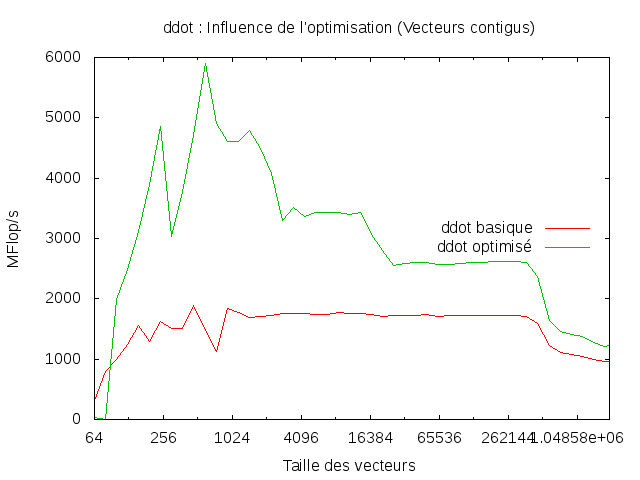
\includegraphics[width=\textwidth]{vec_opt.png}
  \caption{Impact de l'optimisation}
  \label{fig:vec_opt}
\end{subfigure}%
\begin{subfigure}[b]{.5\textwidth}
  \centering
  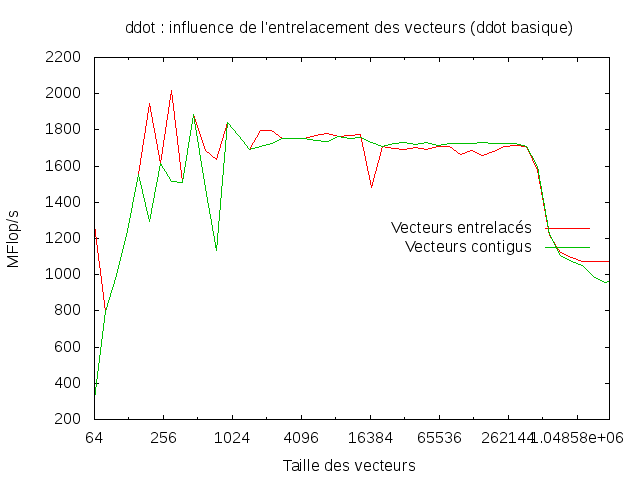
\includegraphics[width=\textwidth]{vec_int.png}
  \caption{Impact de l'entrelacement}
  \label{fig:vec_int}
\end{subfigure}
\begin{subfigure}[b]{.5\textwidth}
  \centering
  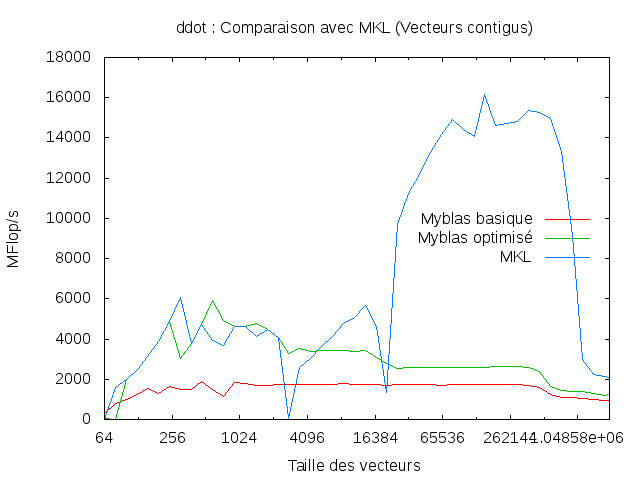
\includegraphics[width=\textwidth]{vec_mkl.png}
  \caption{Comparaison avec MKL}
  \label{fig:vec_mkl}
\end{subfigure}
\caption{Benchmarks pour \texttt{ddot}}
\label{fig:graph_vec}
\end{figure}

La figure \ref{fig:vec_opt} présente les courbes de performances des deux routines implémentées, avec et sans optimisation. 

La figure \ref{fig:vec_int} présente les courbes de performances de notre routine basique selon la distribution des vecteurs en mémoire. On oppose la distribution contiguë ($X_1\cdots X_nY_1\cdots Y_n$) en mémoire à la distribution entrelacée ($X_1Y_1\cdots X_nY_n$). Les autres \emph{benchmarks} sont effectués avec des vecteurs contigus.

La figure \ref{fig:vec_mkl} compare nos algorithmes à la bibliothèque MKL.

\subsubsection{Influence de la taille des vecteurs}

Sur toutes les courbes de la figure \ref{fig:graph_vec}, les performances sont mauvaises lorsque $N$ est très petit ($<100$). Cela est probablement dû aux temps de calculs trop courts qui ne permettent pas de négliger les opération périphériques, telles que les appels de fonctions ou le mécanisme de mesure de temps. Il peut aussi s'agir de l'effet pipeline qui n'intervient que lorsque $N$ est assez grand.
    
On remarque aussi toujours une chute de performances autour de $10^6$, qui se trouve être l'ordre de grandeur du cache L3 (8MB). Dans le même ordre d'idée, sur certaines courbes des creux apparaissent aux alentours de 1000, ce qui est comparable à la taille des caches L1 du processeur (32KB).

\subsubsection{Influence de l'optimisation}

La figure \ref{fig:vec_opt} montre que pour des vecteurs contigus la version optimisée est bien plus rapide que la version basique.
    
Pour $N$ compris entre $10^2$ et $10^4$, les performances sont bien plus élevées, avec une accélération de l'ordre de 4. Entre $10^4$ et $10^6$ le calcul se fait 2 fois plus vite.
    
Le nombre d'opérations de la version optimisée est comparable à la moitié de la fréquence du processeur (2.66GHz). Ceci est probablement du au fait que cet algorithme effectue une multiplication entière pour une opération flottante (2 multiplications pour l'indice, une addition et une multiplication flottante).
    
L'algorithme optimisé donne des valeurs supérieures à la fréquence du processeur entre $10^2$ et $10^4$. Cela indique que plus d'une unité flottante est utilisée à la fois sur le processeur. Il s'agit probablement d'une optimisation impliquant de la vectorialisation par le compilateur intel ou par le matériel. Au delà de $10^4$ on observe un palier dont la valeur est comparable à la fréquence du processeur, ce qui indique qu'un calcul flottant est effectué par cycle. Le gain de performance entre la version optimisée et la version non optimisée semble logique vis-à-vis de la suppression d'une multiplication entière dans la version optimisée.
    
\subsubsection{Influence de l'entrelacement}

La figure \ref{fig:vec_int} montre que les deux distributions de données donnent des résultats similaires pour l'algorithme non optimisé. Il faut cependant bien remarquer que l'algorithme optimisé ne fonctionne que dans le cas contigu. Il est donc préférable d'avoir des vecteurs contigus.
    
\subsubsection{Comparaison avec MKL}

La figure \ref{fig:vec_mkl} montre que MKL est plus rapide que notre bibliothèque pour des vecteurs assez grand. Vers $10^5$ on obtient des valeurs très proches de la puissance théorique d'un coeur (21.8GFlops), ce qui indique que MKL utilise de façon intensive le processeur, probablement en utilisant des mécanismes comme la vectorialisation et le \emph{prefetching} (car à $10^5$ les données ne rentrent plus dans le cache L1).
\section{Produit matriciel}

Le produit matriciel est une opération de type BLAS3, qui sont des opérations matrice-matrice. Dans cette partie, nous allons détailler notre implémentation du produit matriciel \texttt{dgemm} ainsi que les optimisations que nous avons effectué, puis nous analyserons les résultats des \emph{benchmarks}.

\subsection{Algorithmes}

Nous avons implémenté la routine \texttt{dgemm} qui effectue un produit matriciel, puis nous avons effectué deux optimisations successives: le produit par blocs et la parallélisation.

Trois types d'algorithmes ont été implémentés : plusieurs séquentiels, un par bloc (reposant sur le précédent) et un parallèle (reposant sur les deux précédents). Ils sont applicables à des matrices de taille quelconque, trois dimensions différentes sont donc prises en compte lorsque l'on cherche à calculer $C \leftarrow \alpha op(A) \times B + \beta C$ :
\begin{itemize}
\item $m$ le nombre de lignes dans $op(A)$  et $C$ ;
\item $n$ le nombre de colonnes dans $B$ et $C$ ;
\item $k$ le nombre de colonnes dans $op(A)$ et de ligne dans $B$.
\end{itemize}


\subsubsection{Problème}

\paragraph{Entrées.} La routine prend comme paramètres:
\begin{itemize}
\item une matrice A de taille $K*M$
\item une matrice B de taille $K*N$
\item une matrice A de taille $M*N$
\item 2 \texttt{double} $\alpha$ et $\beta$
\end{itemize}
La routine CBLAS prend d'autres informations pour modifier l'opération effectuée, mais nous ne les détaillerons pas ici. Celles-ci seront fixées afin d'effectuer l'opération décrite.

Chaque matrice est décrite par les informations suivantes:
\begin{itemize}
\item Un pointeur $A$ vers le premier élément,
\item Un nombre de lignes $M$
\item Un nombre de colonnes $N$
\item Une \textit{leading dimension} \texttt{lda}
\end{itemize}
Une matrice est représentée par colonnes en mémoire, et chaque colonne est espacée de \texttt{lda}.


\paragraph{Sortie.} La routine modifie la matrice $C$ de la manière suivante:
\begin{equation}
C=\beta \cdot C + \alpha \cdot A^T \cdot B 
\end{equation}
Cela se traduit au niveau des coefficients $c_{i,j}$ par la formule suivante:
\begin{equation}
c_{i,j} = \beta c_{i,j} + \alpha \sum\limits_{k=1}^n a_{k,i} \cdot b_{k,j}
\end{equation}


\paragraph{Complexité.} La complexité de cette routine en nombre d'opérations flottantes à double précision est:
\begin{equation}
C(m,n,k)=(2\times k-1)\times m\times n
\end{equation}
Des optimisations sur la complexité sont possibles, comme par exemple grâce à l'algorithme de Strassen, mais ce type d'algorithmes ne s'adapte pas bien au considérations pratiques de ce TDP.


\subsubsection{Algorithme de base}

Cet algorithme est le plus proche de la forme mathématique ci-dessus, il se décompose en trois boucles itérant sur les variables $i,j,k$ de cette formule. Du fait du caractère commutatif de l'addition, l'ordre des calculs n'influe pas sur le résultat. Le point à étudier est alors la différence de performance entre les trois possibilités d'agencement de ces boucles : $ijk$, $jik$, $kij$.

On se doute que les boucles les plus intérieures doivent respecter la cohérence spatiale, c'est à dire parcourir les colonnes des matrices. Ainsi, la boucle sur $k$ (colonnes de $A$ et $B$) devra être la plus intérieure. Dans cette situation, on écrit tous les $c_{i,j}$ les uns après les autres, ce qui permet d'accumuler les résultats dans un registre et de n'écrire qu'une fois $c_{i,j}$ en mémoire.

\subsubsection{Blocs}\label{sec:algo_bloc}

L'algorithme par blocs change l'ordre des calculs en découpant les matrices en blocs, puis en effectuant les produits matriciels des sous-blocs indépendamment avec l'algorithme de base dans sa version $jik$. La taille des blocs est configurable selon les 3 dimensions $i,j,k$.

Le but de cette optimisation est d'augmenter la réutilisation des valeurs stockées dans les caches. En effet, lors de l'exécution de la routine, chaque valeur dans les matrices $A$ est lue $N$ fois. Si les matrices multipliées tiennent en cache, une seule lecture en RAM est nécessaire pour chaque élément. Si la matrice est trop grande, les lignes de cache sont écrasées. On espère donc que le produit par blocs optimise ces accès au cache pour des tailles de blocs suffisamment petites pour rentrer dans les caches.

Après les \emph{benchmarks}, nous avons choisi des blocs de taille $M=512 , N=512 , K=1024$, ce qui correspond expérimentalement aux performances qui nous ont paru être les meilleures

\subsubsection{Parallélisme}

La parallélisation du produit matriciel est possible en découpant la matrice $C$ en autant de blocs que de processeurs, puis en effectuant les sous produits indépendamment sur chaque processeur.

Soit $p$ le nombre de processeurs. La matrice $C$ est découpée en $M_B*N_B$ blocs avec $M_B$ et $N_B$ tels que $M_B*N_B = p$ et $M_B - N_B$ minimal \footnote{$M_B$ est le plus grand diviseur de $p$ inférieur à $\sqrt p$}. Les matrices $A$ et $B$ sont découpées respectivement en blocs de $N_B$ et $M_B$ colonnes.

Chaque coeur calcule indépendamment son sous-produit matriciel avec l'algorithme par blocs.

\subsection{Benchmark}

Nous avons mesuré les performances des différents algorithmes que nous avons implémenté en faisant varier la taille des données en gardant toujours la même distribution en mémoire.

Toutes les matrices utilisées sont carrées de taille $N$ et remplies aléatoirement. L'espace mémoire est réutilisé, les données accédées peuvent donc rester en cache. On utilise 3 espaces de stockage et on garde toujours la même \emph{leading dimension}, ce qui n'est pas forcément bon pour la localité spatiale.

\begin{figure}[!ht]
\centering

\begin{subfigure}[b]{.5\textwidth}
  \centering
  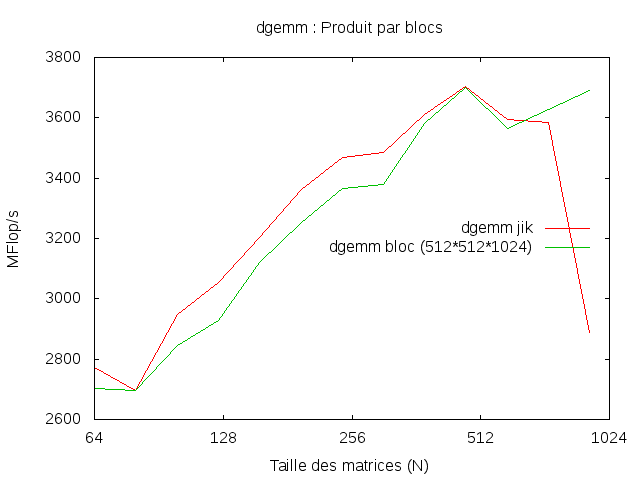
\includegraphics[width=\textwidth]{mat_bloc.png}
  \caption{Optimisation par blocs}
  \label{fig:mat_bloc}
\end{subfigure}%
\begin{subfigure}[b]{.5\textwidth}
  \centering
  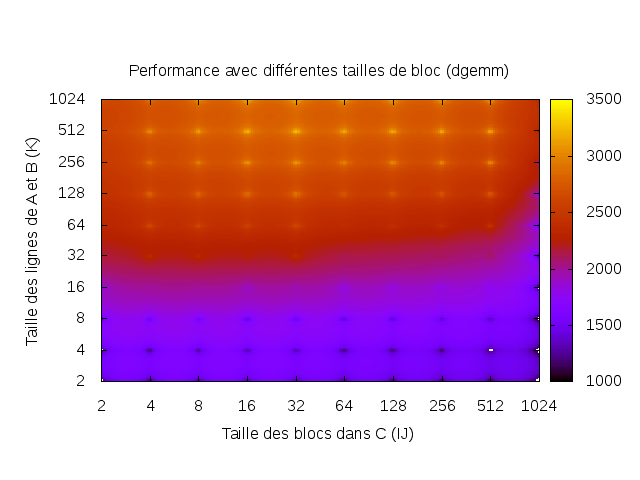
\includegraphics[width=\textwidth]{mat_bloc_size.png}
  \caption{Impact de la taille des blocs}
  \label{fig:mat_bloc_size}
\end{subfigure}

\begin{subfigure}[b]{.5\textwidth}
  \centering
  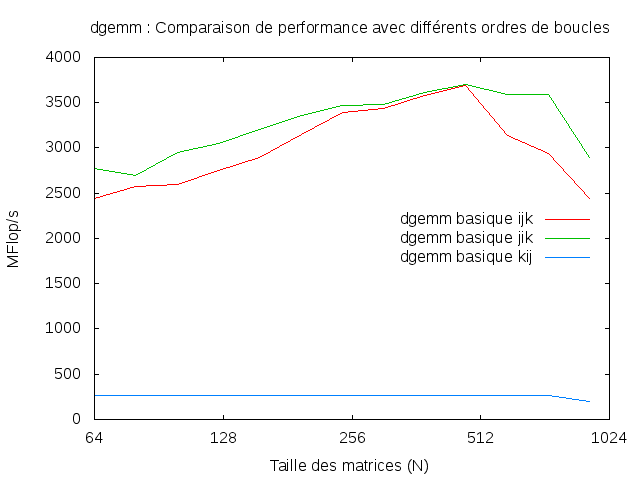
\includegraphics[width=\textwidth]{mat_ijk.png}
  \caption{Impact de l'ordre des boucles}
  \label{fig:mat_ijk}
\end{subfigure}%
\begin{subfigure}[b]{.5\textwidth}
  \centering
  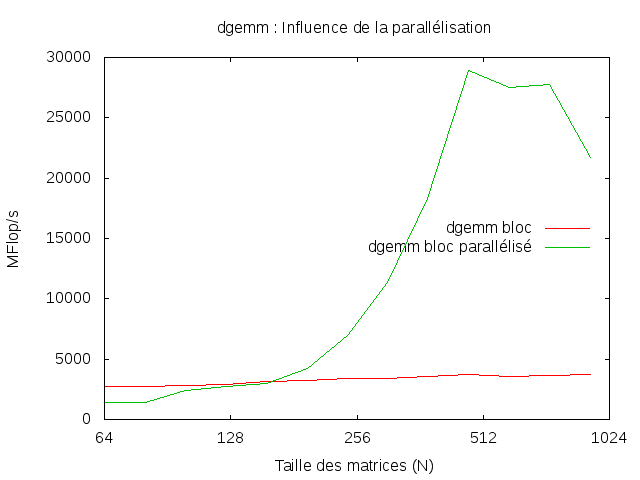
\includegraphics[width=\textwidth]{mat_parallel.png}
  \caption{Résultat de la parallélisation}
  \label{fig:mat_parallel}
\end{subfigure}
\begin{subfigure}[b]{.5\textwidth}
  \centering
  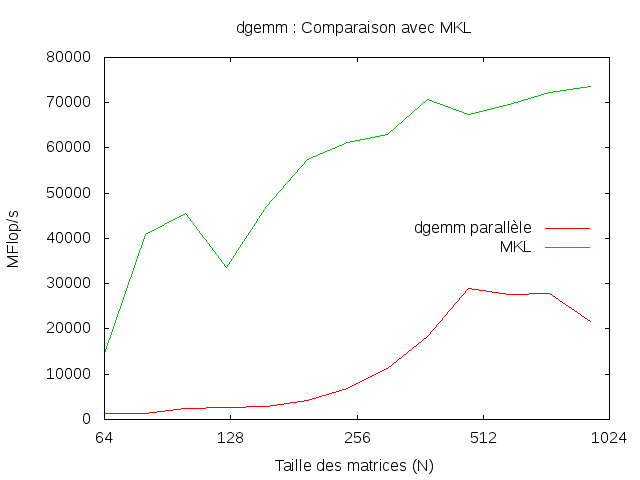
\includegraphics[width=\textwidth]{mat_mkl.png}
  \caption{Comparaison avec MKL}
  \label{fig:mat_mkl}
\end{subfigure}
\caption{Benchmarks pour \texttt{ddot}}
\label{fig:mat}
\end{figure}


\subsubsection{Influence de l'ordre des boucles}

Le graphique \ref{fig:mat_ijk} confirme bien que la boucle su $k$ doit être la plus interne, sinon on perd en performances. Pour l'ordre $kij$ on observe une performance constante d'environ 300 Mflop/s qui correspond probablement à une performance bridée par la bande passante mémoire en écriture dans les $c_{i,j}$.
    
Parcourir les colonnes de $C$ dans la boucle interne ($jik$) donne de légèrement meilleures performances, probablement grâce à la localité spatiale.
    
Les performances augmentent avec les tailles des matrices jusqu'aux environs de $N=512$, au moment ou les matrices remplissent le cache L3 (8Mo).
    
Il est important de noter que ce résultat n'est vrai que lorsque les matrices sont représentées en \texttt{ColMajor} et que $A$ est transposée. On retiendra juste que la boucle la plus interne doit être celle qui préserve la localité spatiale et qui fait toutes les écritures dans un même $c_{i,j}$ à la suite.


\subsubsection{Influence des blocs}

Le graphique \ref{fig:mat_bloc} montre dans quelle mesure le produit par blocs optimise les performances. Les performances sont légèrement moins bonnes jusqu'au moment où le produit $jik$ atteint son maximum de performances. Après ce cap, les performances du produit $jik$ régressent alors que celles du produit bloc restent constantes. Cela est probablement dû au phénomène décrit en \ref{sec:algo_bloc}: le produit bloc réutilise mieux les valeurs en cache.
    
Nous pouvons imaginer que la taille des blocs optimale est atteinte lorsque les blocs remplissent le cache; c'est pourquoi nous avons choisi de découper $C$ en blocs de taille $512*512$ et de prendre des lignes de taille $1024$ afin de garder de la cohérence spatiale.
    
\paragraph{Influence de la taille des blocs}
    
Nous avons aussi voulu montrer quel était l'influence de la taille des blocs sur les performances pour des matrices de taille $1024*1024$. La figure \ref{fig:mat_bloc_size} donne les performances en fonction de deux paramètre: $ij$ la taille des carrés qui composent $C$, et $k$ la taille des lignes dans les matrices $A$ et $B$. 
    
Des points brillants représentent des pics de performances proche des puissances de 2, probablement liés à l'alignement mémoire. On observe que pour avoir de bonnes performances, il faut que les lignes (dimension $K$) soient suffisamment grandes ; sinon les performances sont désastreuses, à l'image de l'algorithme $kij$. Dans ces plages de taille, l'influence de $ij$ n'est pas bien mise en avant, mais le temps de calcul avec des matrices plus grandes devenait trop long. Il semble tout de même que les performances diminuent lorsque $ij$ devient trop grand, et que les points semblent plus brillants lorsque $ij$ est de l'ordre de 32. 
    
L'idéal est donc de prendre des grandes lignes, et de subdiviser $C$ en des matrices plus petites, à priori on a de meilleures performances si les blocs tiennent dans le cache.
    
    
\subsubsection{Influence du parallélisme}

Pour les données sur le parallélisme, le nombre de \emph{threads} créé est de 8.

La figure \ref{fig:mat_parallel} montre le résultat de la parallélisation. Pour des petites tailles, la parallélisation est plus coûteuse que l'algorithme séquentiel, probablement à cause de la mise en place des \emph{threads}. A partir d'une taille de l'ordre de 128 on observe que les performances croissent linéairement en fonction de la taille jusqu'à une taille de 512. L'algorithme est alors à peu près 8 fois plus rapide, ce qui est cohérent avec le nombre de coeurs de la machine.
    
Dans la figure \ref{fig:mat_mkl}, MKL fait 4 fois mieux que notre routine et plafonne à un peu moins de 80 GFlop/s, ce qui semble représenter la puissance crête d'un processeur X5550. Nous nous demandons donc si les 8 \emph{threads} sont distribués sur un seul processeur \emph{hyperthreadé} parmi les 2 processeurs d'un noeud de calcul. Mais nous n'avons pas pu confirmer cette hypothèse.
    
    
\section{Autres routines}

Dans le sujet du TDP, d'autres routines devaient être implémentées, il s'agit de : 
\begin{itemize}
\item \texttt{cblas\_daxpy}, qui calcule l'opération vectorielle $y \leftarrow \alpha x + y$ ;
\item \texttt{cblas\_dgemv}, qui calcule l'opération matrice-veteur $y \leftarrow \alpha op(A)x + \beta y$ ;
\item \texttt{cblas\_dger}, qui calcule l'opération vectorielle $A \leftarrow \alpha xy^{t} + A$.
\end{itemize}

Ces trois BLAS ont été implémentées mais non étudiées.
\section*{Conclusion}
\addcontentsline{toc}{section}{Conclusion}

Nous avons implémenté la simulation du nuage de particules de manière distribuée en utilisant la bibliothèque MPI et analysé les performances de cet algorithme.

Ce qui ressort des benchmarks effectués, est que l'algorithme se parallélise bien car l'accélération obtenue sur une exécution se rapproche fortement du nombre de processeurs. Ce résultat n'est pas étonnant dans la mesure où les calculs (de complexité quadratique) recouvrent rapidement le temps des communications (qui sont de complexité linéaire). 

Différentes techniques ont été mises en \oe uvre pour rendre les communications les plus transparentes possibles, comme la mise en place de communications persistantes et le recouvrement des communications par le calcul. Ces améliorations ont permis d'utiliser les capacités de calcul de manière aussi efficace que l'algorithme séquentiel.

Une autre amélioration à été mise en place, en utilisant un dt variable pour une simulation plus précise. Cette amélioration entraîne cependant un surcoût en temps de calcul.

Des améliorations sont encore possibles, il est notamment possible de diminuer le temps de calcul à chaque itération en optimisant les opérations, mais cela n'entre pas dans le cadre de ce TDP.



\end{document}
